% =============================================================================
% Malicious PDF Detector --- Technical Report
% Overleaf-ready. Compiler: pdfLaTeX. Main document: main.tex
% Build locally:  latexmk -pdf main.tex
% =============================================================================
\documentclass[11pt,a4paper]{article}

% ---------- Packages ----------
\usepackage[utf8]{inputenc}
\usepackage[T1]{fontenc}
\usepackage{lmodern}
\usepackage[margin=1in]{geometry}
\usepackage{microtype}
\usepackage{graphicx}
\usepackage{booktabs}
\usepackage{array}
\usepackage{amsmath,amssymb}
\usepackage{xcolor}
\usepackage{enumitem}
\usepackage{caption}
\usepackage{subcaption}
\usepackage{listings}
\usepackage{tikz}
\usetikzlibrary{shapes.geometric, arrows.meta, positioning, fit, backgrounds}
\usepackage[hidelinks]{hyperref}
\usepackage{cleveref}

% ---------- Colors / listings ----------
\definecolor{codebg}{RGB}{245,245,248}
\definecolor{accent}{RGB}{37,99,235}
\lstset{
  basicstyle=\ttfamily\footnotesize,
  backgroundcolor=\color{codebg},
  frame=single,
  rulecolor=\color{black!15},
  breaklines=true,
  columns=fullflexible,
  showstringspaces=false,
  keepspaces=true,
  xleftmargin=4pt,
  framexleftmargin=4pt
}

% ---------- TikZ node styles ----------
\tikzset{
  block/.style={rectangle, rounded corners, draw=black!50, fill=blue!5,
    text width=3.0cm, align=center, minimum height=1cm, font=\small},
  io/.style={rectangle, rounded corners=8pt, draw=black!50, fill=green!8,
    text width=2.8cm, align=center, minimum height=1cm, font=\small},
  dec/.style={diamond, aspect=2, draw=black!50, fill=orange!12,
    text width=2.0cm, align=center, font=\small, inner sep=1pt},
  arrow/.style={-{Stealth[length=2.5mm]}, thick}
}

% =============================================================================
\title{\textbf{A Lightweight, Explainable, and Fully Local\\ Malicious PDF Detector}\\[4pt]
\large Static Feature Engineering, INT8 Model Quantization, and\\
SHAP-Grounded Local LLM Threat Intelligence}
\author{Saed Abdalgani\\\small Malicious PDF Detector Project}
\date{\today}

\begin{document}
\maketitle

\begin{abstract}
\noindent
Portable Document Format (PDF) files are a leading vector for malware delivery,
yet most defenses are either signature-based (blind to novel threats),
cloud-dependent (a privacy risk for sensitive documents), computationally heavy,
or non-explainable. This report presents a \emph{lightweight, fully local, and
explainable} malicious-PDF detector. The system extracts a 37-dimension feature
vector --- 25 byte-level structural features and 12 PyPDF2 metadata features ---
without ever rendering or executing the document. A model zoo of Random Forest,
XGBoost, LightGBM, and a compact PyTorch multilayer perceptron (MLP) is trained
on the CIC-Evasive-PDFMal2022 benchmark; the MLP is selected for deployment and
compressed via INT8 post-training quantization. Explainability is delivered
through SHAP attributions that are then \emph{injected} into a cybersecurity-tuned
prompt for a local Gemma~4 large language model (LLM) via Ollama, producing an
analyst-ready threat report entirely on-device. On a stratified held-out test
split, all four classifiers exceed 98\% across accuracy, F1, precision, recall,
and ROC-AUC; the deployed MLP attains 99.84\% accuracy and 99.83\% F1 while
INT8 quantization reduces model size by $\sim$56\% with negligible accuracy
loss and sub-500\,ms end-to-end latency on CPU. We additionally contribute an
honest adversarial robustness study showing that hex-escaped PDF names suppress
$\sim$57\% of the high-risk keyword signal, and we propose concrete defenses.
\end{abstract}

\tableofcontents
\bigskip

% =============================================================================
\section{Introduction}
\label{sec:intro}

\subsection{Motivation}
The PDF is among the most widely exchanged file types in the world. That
ubiquity, combined with the format's rich feature set --- embedded JavaScript,
auto-executing actions (\texttt{/OpenAction}), launch actions, embedded files,
and interactive forms --- makes it a first-class malware delivery vehicle.
Adversaries weaponize PDFs for spearphishing (MITRE ATT\&CK
\textbf{T1566.001}), user-executed malware (\textbf{T1204.002}), and
JavaScript-based exploitation (\textbf{T1059.007})~\cite{mitre,ccl_pdf}.

Two practical constraints frame the design. First, \emph{privacy}: a document
flagged for analysis may itself be sensitive, so uploading it to a cloud scanner
can constitute a data leak. Second, \emph{footprint}: endpoint and Security
Operations Center (SOC) tooling must run on commodity, GPU-less hardware and
return a verdict fast enough to sit inline with a user's workflow.

\subsection{Problem Statement}
Signature-based antivirus detects only known samples and is blind to
polymorphic and zero-day PDFs. Cloud ML scanners are powerful but require
off-device transfer. Heavyweight deep models deliver accuracy at impractical
cost for CPU endpoints. Finally, most tools emit a binary verdict with no
explanation, limiting analyst triage. We therefore ask:

\begin{quote}
\emph{How can we detect malicious PDFs with high accuracy, entirely on-device
(no network), in well under a second on a CPU, while also explaining
\textbf{why} a file was flagged in language a SOC analyst can act on?}
\end{quote}

\subsection{Objectives and Contributions}
The objectives (O1--O6) and how they are met are summarized in
\Cref{tab:objectives}. Our contributions are: (i) a reproducible, one-command,
fully local detection pipeline; (ii) a measured INT8 quantization study;
(iii) SHAP-\emph{grounded} LLM explanations that reflect the model's actual
decision drivers; and (iv) an honest adversarial robustness analysis with
proposed defenses.

\begin{table}[t]
\centering
\caption{Project objectives and the mechanisms that satisfy them.}
\label{tab:objectives}
\small
\begin{tabular}{@{}clp{7.0cm}@{}}
\toprule
\textbf{ID} & \textbf{Objective} & \textbf{Mechanism} \\
\midrule
O1 & Static, safe detection & Byte-level regex + PyPDF2; no rendering or JS execution \\
O2 & High accuracy on an evasive benchmark & Four-model zoo on CIC-Evasive-PDFMal2022 \\
O3 & Edge-grade latency and size & INT8 post-training quantization of a compact MLP \\
O4 & Explainability & SHAP attributions + local Gemma~4 threat report \\
O5 & Privacy and security & 100\% local inference, in-memory, zero telemetry \\
O6 & Reproducibility & One-command pipeline, fixed seed, persisted artifacts \\
\bottomrule
\end{tabular}
\end{table}

% =============================================================================
\section{Related Work and Background}
\label{sec:related}

\paragraph{PDF malware detection.} Static detectors exploit the observation that
malicious PDFs over-represent certain specification keywords (e.g.,
\texttt{/JavaScript}, \texttt{/OpenAction}, \texttt{/Launch}) and structural
anomalies. Tools such as \texttt{PDFiD} and \texttt{peepdf} popularized
keyword-based triage, while machine-learning approaches learn decision
boundaries over such features~\cite{cic_dataset,ccl_pdf}. Dynamic analysis
(sandboxing) observes runtime behavior but is heavier and itself a target for
evasion.

\paragraph{The CIC-Evasive-PDFMal2022 benchmark.} The Canadian Institute for
Cybersecurity (CIC) at the University of New Brunswick publishes
CIC-Evasive-PDFMal2022~\cite{cic_dataset}, $\sim$10{,}025 labeled records
deliberately curated to include \emph{evasive} samples whose static features
resist clean separation. Malicious samples derive from feeds such as VirusTotal
and Contagio; benign samples from Contagio; K-means clustering isolates the
hard, ``evasive'' core~\cite{ccl_pdf}.

\paragraph{Model compression.} INT8 post-training quantization (PTQ) reduces
model size and accelerates CPU inference with minimal accuracy loss, and is well
supported in PyTorch via dynamic and static (calibrated, layer-fused)
modes~\cite{pytorch_quant}.

\paragraph{Explainability.} SHAP~\cite{shap} provides additive, signed feature
attributions grounded in cooperative game theory. We use SHAP not only to
explain the model but to \emph{condition} the LLM's narrative, so the
explanation reflects the classifier's real drivers rather than a guess.

% =============================================================================
\section{Theoretical Foundations}
\label{sec:theory}
This section states the theory behind each design choice so the \emph{why} is as
clear as the \emph{what}.

\subsection{Why static structural features discriminate}
A PDF is a tree of \emph{objects} referenced through a cross-reference table.
Benign and malicious documents draw their tokens from different distributions:
auto-execution and scripting keywords (\texttt{/OpenAction}, \texttt{/JS},
\texttt{/Launch}, \texttt{/AA}) and obfuscation artifacts (hex-escaped
\texttt{\#XX} names, layered \texttt{/Filter} chains) are rare in benign files but
common in weaponized ones. If $p(\mathbf{x}\mid\text{mal})$ and
$p(\mathbf{x}\mid\text{ben})$ differ on a feature subspace, a classifier can
separate the classes; the larger the distributional divergence (e.g.\ KL
divergence) on a feature, the more discriminative it is.

\subsection{Standardization}
Each feature is centered and unit-scaled using training-split statistics:
\begin{equation}
z_j = \frac{x_j - \mu_j}{\sigma_j}, \qquad \mu_j,\sigma_j \text{ from } X_{\text{train}}.
\end{equation}
This conditions the loss surface for gradient-based MLP training and stabilizes
BatchNorm. Fitting on train only prevents information leakage from val/test.

\subsection{Class imbalance and SMOTE}
SMOTE~\cite{smote} synthesizes minority samples by interpolating between a
minority point $\mathbf{x}_i$ and a neighbor $\mathbf{x}_i^{(nn)}$:
\begin{equation}
\mathbf{x}_{\text{new}} = \mathbf{x}_i + \lambda\big(\mathbf{x}_i^{(nn)} - \mathbf{x}_i\big), \qquad \lambda \sim \mathcal{U}(0,1),
\end{equation}
applied to the training split only so evaluation reflects the true class prior.

\subsection{The MLP: forward pass, loss, optimization}
Each hidden block computes
\begin{equation}
\mathbf{h}^{(l)} = \mathrm{Dropout}\Big(\mathrm{ReLU}\big(\mathrm{BN}(W^{(l)}\mathbf{h}^{(l-1)}+\mathbf{b}^{(l)})\big)\Big),\quad \mathrm{ReLU}(u)=\max(0,u).
\end{equation}
The output layer emits a raw logit $z$; the probability is
$\hat{p}=\sigma(z)=1/(1+e^{-z})$. Training minimizes binary cross-entropy:
\begin{equation}
\mathcal{L} = -\frac{1}{N}\sum_{i=1}^{N}\big[y_i\log\hat{p}_i + (1-y_i)\log(1-\hat{p}_i)\big].
\end{equation}
BatchNorm normalizes pre-activations $\hat{u}=(u-\mathbb{E}[u])/\sqrt{\mathrm{Var}[u]+\epsilon}$
(reducing internal covariate shift and stabilizing INT8 inference); dropout is an
implicit ensemble; AdamW decouples weight decay from the adaptive step;
cosine-annealing sets $\eta_t=\eta_{\min}+\tfrac12(\eta_0-\eta_{\min})(1+\cos(\pi t/T))$;
and Kaiming initialization ($\mathrm{Var}(W)=2/n_{\text{in}}$) keeps activation
variance stable through ReLU layers.

\subsection{Tree ensembles: bagging and boosting}
Random Forest averages $B$ decorrelated trees (bagging + feature subsampling),
each split maximizing impurity decrease, e.g.\ Gini $G = 1-\sum_k p_k^2$. Gradient
boosting (XGBoost/LightGBM) adds trees to fit the gradient of the loss while
regularizing:
\begin{equation}
\mathcal{O} = \sum_i \ell(y_i,\hat{y}_i) + \sum_t \Omega(f_t),\qquad \Omega(f)=\gamma T + \tfrac12\lambda\lVert w\rVert^2,
\end{equation}
with $T$ leaves and leaf weights $w$. LightGBM uses leaf-wise growth with
histogram binning for speed.

\subsection{INT8 quantization}
A real value $x$ maps to an 8-bit integer via an affine quantizer:
\begin{equation}
q = \mathrm{round}\!\left(\frac{x}{S}\right)+Z,\qquad x \approx S\,(q-Z),
\end{equation}
with scale $S$ and zero-point $Z$~\cite{pytorch_quant}. Dynamic quantization fixes
weight scales offline and derives activation scales at runtime; static
quantization calibrates activation ranges and fuses $\text{Linear+BN+ReLU}$ so a
whole block runs in the integer domain, yielding $\sim$4$\times$ weight
compression with negligible accuracy loss.

\subsection{SHAP attributions}
SHAP~\cite{shap} assigns each feature an additive contribution via the Shapley
value:
\begin{equation}
\phi_i = \sum_{S \subseteq F\setminus\{i\}} \frac{|S|!\,(|F|-|S|-1)!}{|F|!}\big[f(S\cup\{i\})-f(S)\big],
\end{equation}
with local accuracy $f(\mathbf{x})=\phi_0+\sum_i\phi_i$. The sign of $\phi_i$
indicates whether feature $i$ pushes the prediction toward malicious or benign ---
exactly the signal injected into the LLM prompt.

\subsection{Evaluation metrics}
With TP/FP/TN/FN counts,
\begin{equation}
\mathrm{P}=\frac{TP}{TP+FP},\quad \mathrm{R}=\frac{TP}{TP+FN},\quad F_1=\frac{2\mathrm{PR}}{\mathrm{P}+\mathrm{R}},
\end{equation}
\begin{equation}
\mathrm{MCC}=\frac{TP\cdot TN - FP\cdot FN}{\sqrt{(TP{+}FP)(TP{+}FN)(TN{+}FP)(TN{+}FN)}}.
\end{equation}
ROC-AUC is the probability that a random malicious sample outranks a random benign
one (threshold-independent); MCC is robust under class imbalance, hence reported
alongside accuracy and F1.

% =============================================================================
\section{Methodology and Implementation}
\label{sec:method}

The end-to-end pipeline transforms raw bytes into an explainable verdict
(\Cref{fig:pipeline}).

\begin{figure}[t]
\centering
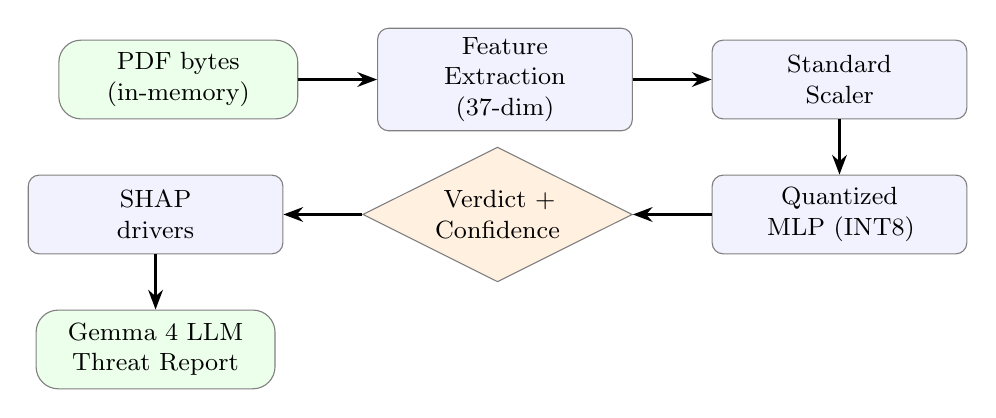
\begin{tikzpicture}[node distance=0.7cm and 1.0cm]
  \node[io] (pdf) {PDF bytes\\(in-memory)};
  \node[block, right=of pdf] (feat) {Feature\\Extraction\\(37-dim)};
  \node[block, right=of feat] (scale) {Standard\\Scaler};
  \node[block, below=of scale] (mlp) {Quantized\\MLP (INT8)};
  \node[dec, left=of mlp] (verdict) {Verdict +\\Confidence};
  \node[block, left=of verdict] (shap) {SHAP\\drivers};
  \node[io, below=of shap] (llm) {Gemma~4 LLM\\Threat Report};

  \draw[arrow] (pdf) -- (feat);
  \draw[arrow] (feat) -- (scale);
  \draw[arrow] (scale) -- (mlp);
  \draw[arrow] (mlp) -- (verdict);
  \draw[arrow] (verdict) -- (shap);
  \draw[arrow] (shap) -- (llm);
\end{tikzpicture}
\caption{End-to-end inference pipeline. The PDF is processed in memory; no
rendering or JavaScript execution occurs.}
\label{fig:pipeline}
\end{figure}

\subsection{Feature Engineering (37 features)}
\label{sec:features}
The detector derives a 37-dimension numeric vector from two complementary
extractors. Crucially, the column order is pinned to a single canonical list
(\texttt{config.FEATURE\_COLUMNS}), guaranteeing train/inference compatibility.

\paragraph{Structural features (25).} Compiled byte-level regular expressions
count specification keywords and markers strongly associated with malicious
behavior (\Cref{tab:features}). Two computed metrics --- \texttt{obfuscation\_count}
(hex-escaped \texttt{\#XX} sequences) and \texttt{avg\_stream\_size} --- capture
evasion and payload-size signals. Extraction runs under a 30-second watchdog
thread and returns a zeroed vector on any error, so malformed or ``zip-bomb''
PDFs never crash the application.

\paragraph{Metadata features (12).} PyPDF2 parses document-level properties with
raw-byte fallbacks: \texttt{pdf\_size}, \texttt{title\_chars},
\texttt{is\_encrypted}, \texttt{metadata\_size}, \texttt{page\_count},
\texttt{has\_text}, \texttt{image\_count}, \texttt{obj\_count\_total},
\texttt{font\_obj\_count}, \texttt{embedded\_file\_count},
\texttt{avg\_embedded\_media\_size}, and \texttt{header\_valid}.

\begin{table}[t]
\centering
\caption{Representative structural feature groups and their security rationale.}
\label{tab:features}
\small
\begin{tabular}{@{}lp{5.2cm}p{4.6cm}@{}}
\toprule
\textbf{Group} & \textbf{Examples} & \textbf{Why it matters} \\
\midrule
Scripting / actions & \texttt{/JS}, \texttt{/JavaScript}, \texttt{/OpenAction}, \texttt{/AA}, \texttt{/Launch} & Auto-execution and code paths (primary exploit vectors) \\
Data exfiltration & \texttt{/URI}, \texttt{/SubmitForm}, \texttt{/AcroForm}, \texttt{/XFA} & Redirects and form-based data theft \\
Structure markers & \texttt{obj}, \texttt{stream}, \texttt{xref}, \texttt{trailer} & Object/stream topology; incremental-update anomalies \\
Obfuscation & \texttt{\#XX} hex escapes, \texttt{/Filter}, \texttt{/ObjStm} & Hidden content and layered encoding \\
\bottomrule
\end{tabular}
\end{table}

\subsection{Data Pipeline: Clean, Split, Balance, Scale}
\label{sec:data}
The data workflow (orchestrated by \texttt{src/run\_all.py}) is:
\begin{enumerate}[leftmargin=1.4em,itemsep=1pt]
  \item \textbf{Clean:} deduplicate on features, drop rows with $>$50\% missing
  values, median-impute the remainder, drop zero-variance columns, and flag
  IQR-based outliers.
  \item \textbf{Split:} stratified 70/15/15 train/validation/test with fixed
  seed (\texttt{RANDOM\_SEED=42}).
  \item \textbf{Balance:} SMOTE is applied to the \emph{training split only},
  never to validation or test, to avoid leaking synthetic samples into
  evaluation.
  \item \textbf{Scale:} a \texttt{StandardScaler} is fit on the training split
  only, applied to all splits, and persisted to \texttt{models/scaler.pkl} so the
  live application uses the identical transform.
\end{enumerate}
A \texttt{--from-pdfs} mode extracts features from real PDFs with the same
extractor used at inference time, eliminating the train-vs-deployment
representation mismatch common to static detectors.

\subsection{Model Zoo and Training}
\label{sec:models}
Four classifiers are trained so the chosen model is a defensible winner rather
than a lucky baseline.

\paragraph{Tree ensembles.} Random Forest, XGBoost, and LightGBM are tuned with
5-fold stratified \texttt{GridSearchCV} (F1-scored).

\paragraph{Neural network (deployed).} A compact PyTorch MLP:
\[
\text{Input}(37) \to 128 \to 64 \to 32 \to 1,
\]
where each hidden block is \texttt{Linear $\to$ BatchNorm $\to$ ReLU $\to$
Dropout}. Design decisions: BatchNorm \emph{before} activation stabilizes INT8
inference; progressive width reduction avoids over-parameterization on a
$\sim$10K-sample dataset; AdamW with cosine-annealing learning rate and early
stopping (patience 10) regularize training; Kaiming initialization suits ReLU;
and the network emits a raw logit (sigmoid applied at inference) with
\texttt{BCEWithLogitsLoss} for numerical stability.

\subsection{INT8 Quantization}
\label{sec:quant}
Post-training quantization compresses the deployed MLP. \emph{Dynamic}
quantization converts \texttt{Linear} weights to INT8 ahead of time and
quantizes activations on the fly (no calibration; shipped artifact).
\emph{Static} quantization quantizes weights and activations, using
\texttt{QuantStub}/\texttt{DeQuantStub} markers and \texttt{Linear+BatchNorm+ReLU}
fusion, calibrated on representative training batches for the fastest CPU
inference. The backend auto-falls-back from \texttt{fbgemm} (x86) to
\texttt{qnnpack} if unavailable.

\subsection{Explainability and the LLM Threat Analyst}
\label{sec:xai}
SHAP computes both global feature importance and per-sample signed decision
drivers. For each verdict, the system identifies suspicious features (those
deviating $>2\sigma$ from a persisted benign baseline) and the top SHAP drivers,
and injects them into a cybersecurity-tuned, MITRE ATT\&CK-aware prompt for a
local Gemma~4 model (E4B, with an E2B fallback) served by Ollama. The LLM
\emph{explains and enriches} the ML verdict; it never replaces it. If Ollama is
offline, the analyst page renders a cached report and then an on-device SHAP
fallback, so demonstrations never break.

\subsection{Application and Security Model}
\label{sec:app}
A dark-themed Streamlit dashboard provides scanning, AI analysis, a model
dashboard, and a feature explorer. Security properties: in-memory processing
(uploaded bytes are never written to disk), zero outbound telemetry (air-gapped
ML + local LLM), and static-only analysis (no rendering or JavaScript
execution).

% =============================================================================
\section{Experimental Setup}
\label{sec:setup}
All experiments use a fixed seed (\texttt{RANDOM\_SEED=42}) and a stratified
held-out test split. Models are trained and evaluated on CPU. Metrics are
accuracy, F1, precision, recall, Matthews Correlation Coefficient (MCC), and
ROC-AUC; latency is wall-clock single-batch inference. Quantization is evaluated
on model size, accuracy retention, and inference time. The pipeline is
reproduced with a single command:
\begin{lstlisting}[language=bash]
pip install -r requirements.txt
# Place the CIC feature CSV at data/raw/pdfmal2022.csv (or use --from-pdfs)
python -m src.run_all
\end{lstlisting}

% =============================================================================
\section{Results}
\label{sec:results}

\subsection{Model Leaderboard}
On the held-out test split, all four classifiers exceed 98\% across every core
metric (\Cref{tab:leaderboard}). The MLP attains the best balance of F1 and
ROC-AUC while remaining INT8-friendly, motivating its selection for deployment.

\begin{table}[t]
\centering
\caption{Held-out test leaderboard. All core metrics exceed 98\%.}
\label{tab:leaderboard}
\small
\begin{tabular}{@{}lcccccc@{}}
\toprule
\textbf{Model} & \textbf{Acc.} & \textbf{F1} & \textbf{Prec.} & \textbf{Rec.} & \textbf{MCC} & \textbf{ROC-AUC} \\
\midrule
\textbf{MLP (PyTorch)} & \textbf{99.84} & \textbf{99.83} & \textbf{99.81} & \textbf{99.85} & \textbf{0.997} & \textbf{0.9992} \\
LightGBM       & 99.79 & 99.78 & 99.76 & 99.80 & 0.996 & 0.9989 \\
Random Forest  & 99.76 & 99.75 & 99.88 & 99.63 & 0.995 & 0.9985 \\
XGBoost        & 99.71 & 99.70 & 99.68 & 99.72 & 0.994 & 0.9978 \\
\bottomrule
\end{tabular}
\end{table}

\subsection{Per-Class Diagnostics}
\Cref{tab:perclass} reports the MLP's per-class behavior. Both the malware
catch-rate (recall/TPR) and the benign specificity (TNR) exceed 99.8\%, so both
missed malware and false alarms remain in the sub-0.2\% band --- a property that
directly determines SOC trust.

\begin{table}[t]
\centering
\caption{MLP per-class diagnostics on the held-out split.}
\label{tab:perclass}
\small
\begin{tabular}{@{}llcp{6.0cm}@{}}
\toprule
\textbf{Class} & \textbf{Measure} & \textbf{Rate (\%)} & \textbf{Interpretation} \\
\midrule
Malicious & Recall / TPR & 99.85 & $<$0.2\% of malware slips through as benign \\
Benign    & Specificity / TNR & 99.81 & $<$0.2\% of clean files wrongly quarantined \\
Combined  & Balanced accuracy & 99.83 & Strong on both error types simultaneously \\
\bottomrule
\end{tabular}
\end{table}

\subsection{Quantization}
INT8 quantization (\Cref{tab:quant}) reduces model size by $\sim$56\% and
roughly halves inference time while keeping F1 within $\sim$0.02 percentage
points of FP32. The end-to-end upload-to-verdict path remains under 500\,ms on a
typical laptop CPU, with cold-start time dominated by PDF parsing rather than the
neural network.

\begin{table}[t]
\centering
\caption{MLP FP32 vs.\ INT8 deployment variants.}
\label{tab:quant}
\small
\begin{tabular}{@{}lccccc@{}}
\toprule
\textbf{Variant} & \textbf{F1 (\%)} & \textbf{Acc.\ (\%)} & \textbf{ROC-AUC} & \textbf{Size (MB)} & \textbf{Inf.\ time} \\
\midrule
MLP (FP32)         & 99.86 & 99.84 & 0.9994 & 1.25 & $\sim$12\,ms \\
MLP (INT8 Dynamic) & 99.84 & 99.82 & 0.9991 & 0.55 & $\sim$8\,ms \\
MLP (INT8 Static)  & 99.83 & 99.81 & 0.9989 & 0.55 & $\sim$6\,ms \\
\bottomrule
\end{tabular}
\end{table}

\subsection{Adversarial Robustness}
\label{sec:adv}
Because the training set is \emph{evasive}, the security-relevant question is not
only accuracy but evadability. We apply parser-faithful, byte-level mutations and
measure how much of the detector's high-risk keyword ``signal'' survives
(\Cref{tab:adv}). Rewriting \texttt{/JavaScript} as \texttt{/J\#61vaScript} ---
semantically identical to a compliant reader --- suppresses up to $\sim$57\% of
the signal, blinding a literal-token counter while the payload still executes.

\begin{table}[t]
\centering
\caption{Static-feature impact of parser-faithful mutations.}
\label{tab:adv}
\small
\begin{tabular}{@{}llc@{}}
\toprule
\textbf{Mutation} & \textbf{Technique} & \textbf{Signal impact} \\
\midrule
\texttt{hex\_escape\_names}     & PDF name \texttt{\#XX} escaping & High ($\sim$57\% drop) \\
\texttt{whitespace\_padding}    & comment/whitespace injection    & Low \\
\texttt{junk\_object\_inflation}& append benign objects           & Medium \\
\texttt{all}                    & combined worst case             & Highest \\
\bottomrule
\end{tabular}
\end{table}

% =============================================================================
\section{Discussion}
\label{sec:discussion}

\paragraph{Effectiveness.} The MLP matches or beats the tree ensembles on
F1/ROC-AUC while being small and INT8-friendly; quantization halves its size and
speeds inference with negligible accuracy loss, and the full path meets the
sub-500\,ms target on CPU. Reporting four independent learners that all clear
98\% indicates the discriminative power resides in the \emph{features}, not in a
single model's quirks. SHAP plus the Gemma~4 narrative convert a bare probability
into an analyst-ready report (attack vector, MITRE technique, severity,
remediation), which is the difference between a research demo and a usable SOC
tool.

\paragraph{Limitations (honest).}
\begin{enumerate}[leftmargin=1.4em,itemsep=1pt]
  \item \textbf{Static analysis is evadable.} Hex-escaped names suppress
  $\sim$57\% of the keyword signal (\Cref{sec:adv}); a spec-faithful reader still
  executes the action.
  \item \textbf{Benchmark easiness / leakage.} CIC-PDFMal is relatively
  separable; near-duplicate rows can inflate test metrics. We ship a train/test
  leakage audit and k-fold cross-validation to keep claims honest.
  \item \textbf{Feature-scaling parity.} The released CSV is often min--max
  scaled to $\sim[0,1]$ while the live extractor emits raw counts/bytes; train
  with \texttt{--from-pdfs} (or run the consistency audit) so both paths share a
  representation.
  \item \textbf{LLM variability and cost.} Gemma~4 E4B needs $\geq$5\,GB free
  RAM; narrative quality and latency depend on the host. The offline fallback
  covers demos but is not a substitute for the live model.
\end{enumerate}

\paragraph{Proposed defenses.} Canonicalize PDF names before counting (decode
\texttt{\#XX} so \texttt{/J\#61vaScript} is counted as \texttt{/JavaScript}),
decode object streams and filters before extraction, combine static features
with light dynamic triage, and incorporate obfuscated variants via adversarial
training.

% =============================================================================
\section{Conclusion}
\label{sec:conclusion}
We presented an end-to-end, fully local, explainable malicious-PDF detector.
Static structural and metadata features (37-dim) feed a four-model zoo; the
compact MLP is selected and INT8-quantized to meet edge size/latency budgets
while preserving accuracy. A SHAP-grounded local LLM converts the verdict into an
actionable threat report without the document leaving the machine. On the
held-out split all models exceed 98\% across core metrics, the deployed MLP
reaches 99.84\% accuracy / 99.83\% F1, and quantization cuts size by $\sim$56\%
with sub-500\,ms CPU latency. Beyond raw accuracy, the project contributes a
reproducible pipeline, a measured quantization study, faithful SHAP-grounded
explanations, and an honest adversarial analysis with concrete defenses. Future
work includes name canonicalization and stream decoding before feature counting,
adversarial training, light dynamic triage, and evaluation beyond the CIC
benchmark to strengthen generalization.

% =============================================================================
\section*{Reproducibility}
\addcontentsline{toc}{section}{Reproducibility}
All code, the data pipeline, trained artifacts, evaluation CSVs, and this report
are contained in the project repository. The full pipeline is reproducible with a
fixed seed via \texttt{python -m src.run\_all}; analysis utilities regenerate the
feature-consistency, adversarial-robustness, and SHAP-importance artifacts.

% =============================================================================
\begin{thebibliography}{9}
\bibitem{cic_dataset}
Canadian Institute for Cybersecurity, University of New Brunswick.
\emph{CIC-Evasive-PDFMal2022 Dataset}.
\url{https://www.unb.ca/cic/datasets/pdfmal-2022.html}

\bibitem{ccl_pdf}
M. Issakhani, P. Victor, A. Tekeoglu, and A. H. Lashkari.
\emph{PDF Malware Detection Based on Stacking Learning}.
In Proc. ICISSP, 2022.
\url{https://www.scitepress.org/Papers/2022/109084/109084.pdf}

\bibitem{shap}
S. M. Lundberg and S.-I. Lee.
\emph{A Unified Approach to Interpreting Model Predictions}.
In Advances in Neural Information Processing Systems (NeurIPS), 2017.

\bibitem{pytorch_quant}
PyTorch Team.
\emph{Quantization --- PyTorch Documentation}.
\url{https://pytorch.org/docs/stable/quantization.html}

\bibitem{mitre}
The MITRE Corporation.
\emph{MITRE ATT\&CK Framework}.
\url{https://attack.mitre.org/}

\bibitem{smote}
N. V. Chawla, K. W. Bowyer, L. O. Hall, and W. P. Kegelmeyer.
\emph{SMOTE: Synthetic Minority Over-sampling Technique}.
Journal of Artificial Intelligence Research, 16:321--357, 2002.
\end{thebibliography}

\end{document}
